\section{Software}

To actually test the FPGA implementation of the neural network with data an effective software interface which handles the processing is needed. It should ease the sending of single or multiple images to the FPGA, control and handle the execution of it and collect the estimated results. This software should also take take care that the input data is processed in right order and arriving input images should be effectively queued to prevent errors from evaluating multiple images at once. Further the software should also handle any necessary high level tasks which are needed, e.g. the support of common image datatypes and their conversion to a suitable representation.

Another important target is that the network should have an interface to Python because it emerged to a de-facto standard in the Neural Network, Machine Learning Scientific community \cite{Virtanen:2020aa}. All the major development in Machine Learning is done in Python and because the Zedboard is able to run Linux and Python an implementation is possible.
In the long term it would also be beneficial to control the network via Python and embed it in an existing Machine Learning Framework like Keras \cite{Gulli:2017aa} or Torch \cite{Paszke:2019aa}. This would enable an high level usage of FPGAs for neural network hardware acceleration. 

Besides from the \gls{acr:ML} tasks the sparse resources of the Zedboard are conserved as much as possible. Therefore no \gls{acr:GUI} is implemented and communication happens exclusively via textual interfaces, e.g. Serial Connections or Ethernet. Transferring data of these textual interfaces is tedious which why also webapp is implemented as a compromise of ease of use and resource consumption.

The overall goals of the software layer therefore can be summarized as:

\begin{itemize}
	\item Write a low level driver in C to communicate with the FPGA
	\item Provide a Python Interface to the driver
	\item Provide a Web control interface
\end{itemize}


\subsection{FPGA Driver}

The user layer driver software implements an interface between the ARM Top-Level software and the driver for the programmable logic. It directly uses the Linux driver \gls{acr:API} and and is implemented in C. It is supposed to handle the entire communication with the driver so that the hardware is only abstractly visible for the ARM Top-Level software. It is build on top of the Xilinx FPGA driver. \\
\noindent
An important task that needs to handled by the driver is the synchronization of the FPGA and Linux. We use the POSIX standard \emph{pthread} library which provides routines for mutual exclusion to ensure that the FPGA is not accessed from multiple threads at the same time. Further the driver communicates with the low-level Xilinx driver using the function \texttt{ioctl()} which blocks the thread until the releasing hardware interrupt occurs. In our case the blocking of the thread is acceptable because multithreading is handled on a higher abstraction level. Copying of the data from user space to the FPGA is done via the C function\footnote{Note: Still the driver need to check that not multiple threads access it at the same time.}. \\
Control and debug data is transferred via AXI-lite bus using UIO-device driver. It maps the corresponding AXI-lite bus address to a virtual memory address. This address can be used to read or write from the AXI-lite device. 

\begin{figure}[hbt]
  \centering
  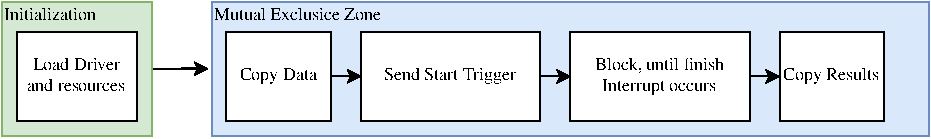
\includegraphics[width=0.8\textwidth]{img/eggdriver.pdf}
  \caption{The network driver}
  \label{fig:sw-python-eggdriver-build}
\end{figure}

Requirements of the User Layer Driver Software:
\begin{itemize} 
	\item Communication with the kernel space drivers 
	\item Easy to use interface from Top-Level 
	\item No knowledge of the hardware should be necessary to use the interface
	\item Data encapsulation to avoid the Top-Level Software from corrupting the memory 
	\item Ability to debug the network, e.g. receive data from the intermediate layers
\end{itemize}

\subsection{Python Driver Interface}
\label{sec:sw-python}

The Python driver interface is build on top of the \gls{acr:FPGA} driver and should ease the usage of the driver functions for the python interface. A very common library and part of the scientific python package is \emph{NumPy} \cite{Virtanen:2020aa}. It's basic element is the \emph{NumPy Array} \cite{Walt:2011aa} which is a very useful abstraction and interface to high dimensional data used in \gls{acr:ML} contexts and a basic building block in most numeric scientific python programs. The Python driver should therefore receive NumPy arrays on the Python side and translate them for the C driver interface. 
This translation process can be automated by tools like e.g. \emph{SWIG} \cite{Beazley:2003aa}.	The (simplified) build process is depicted in Figure~\ref{fig:sw-python-eggdriver-build} which on its basis requires two files: 
First, a header file which contains the C function declearations that should be wrapped, which is the public interface of our driver and second, a special \emph{SWIG} interface files, which contains further rules how the code in the header file should be wrapped. It is often beneficial to create the function declarations in the header files with Python and SWIG in mind. 
SWIG translates the function declarations to the Python domain and creates a \texttt{.py} file with convenience function definitions and a \texttt{.c} file which handles the communication between the C library and (C-)Python. The compilation of this file requires linking against platform specific libraries of the driver, the C library and Python. The whole process is done most conveniently via the Python Setuptools.

\begin{figure}[hbt]
  \centering
  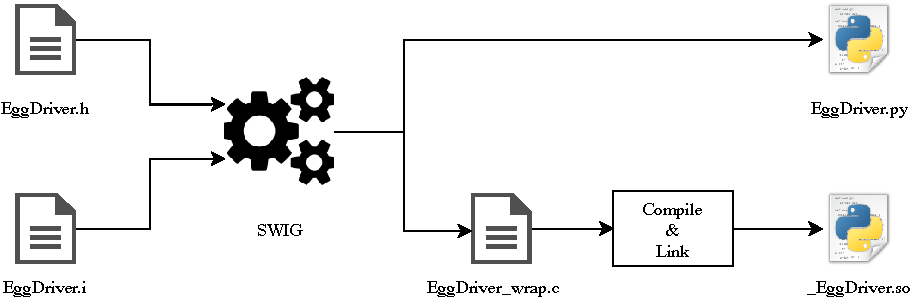
\includegraphics[width=0.8\textwidth]{img/pydriver.pdf}
  \caption{Build process of the Python Driver Interface (simplified)}
  \label{fig:sw-python-eggdriver-build}
\end{figure}


\subsection{Web Interface}

The Webapp should provide an easy yet practical interface to control the network and check its functionality. Because most of the networks software logic is done in Python, also the backend of the Webapp was done with \emph{Python Flask} \cite{Pallets:2020aa}. This enabled us the quick interfacing between web components and our python code and also made the communication of multiple threads easier.

The network speed can be tested and benchmarked to the CPU version (using floats or integers), see the Screenshot in Figure~\ref{fig:sw-webapp-bench}. Here different (sub-)datasets can be chosen as well as different batch sizes. It is also possible to upload a single image in various formats which is then resized to $28 \times 28$ pixels and converted to a NumPy array, which is ultimately transferred to the \gls{acr:FPGA}. Additionally the Webapp automatically queries system status information and displays them using interactive graphs. Most of the functionality is implemented using JavaScript and supporting libraries, e.g. \emph{Chart.js} and \emph{Vue.js}. This is very resource sparse because most of the work is done in the client web browser and only the \gls{acr:API} queries as well as the \gls{acr:NN} must be processed by the Zedboard.

Initially planned but \emph{not} implemented was a possibility of updating of the bitstream via the Webapp. This would have enabled to quickly benchmark various architectures against each other as long as the all conform to common driver interface.

\begin{figure}[hbtp]
  \centering
  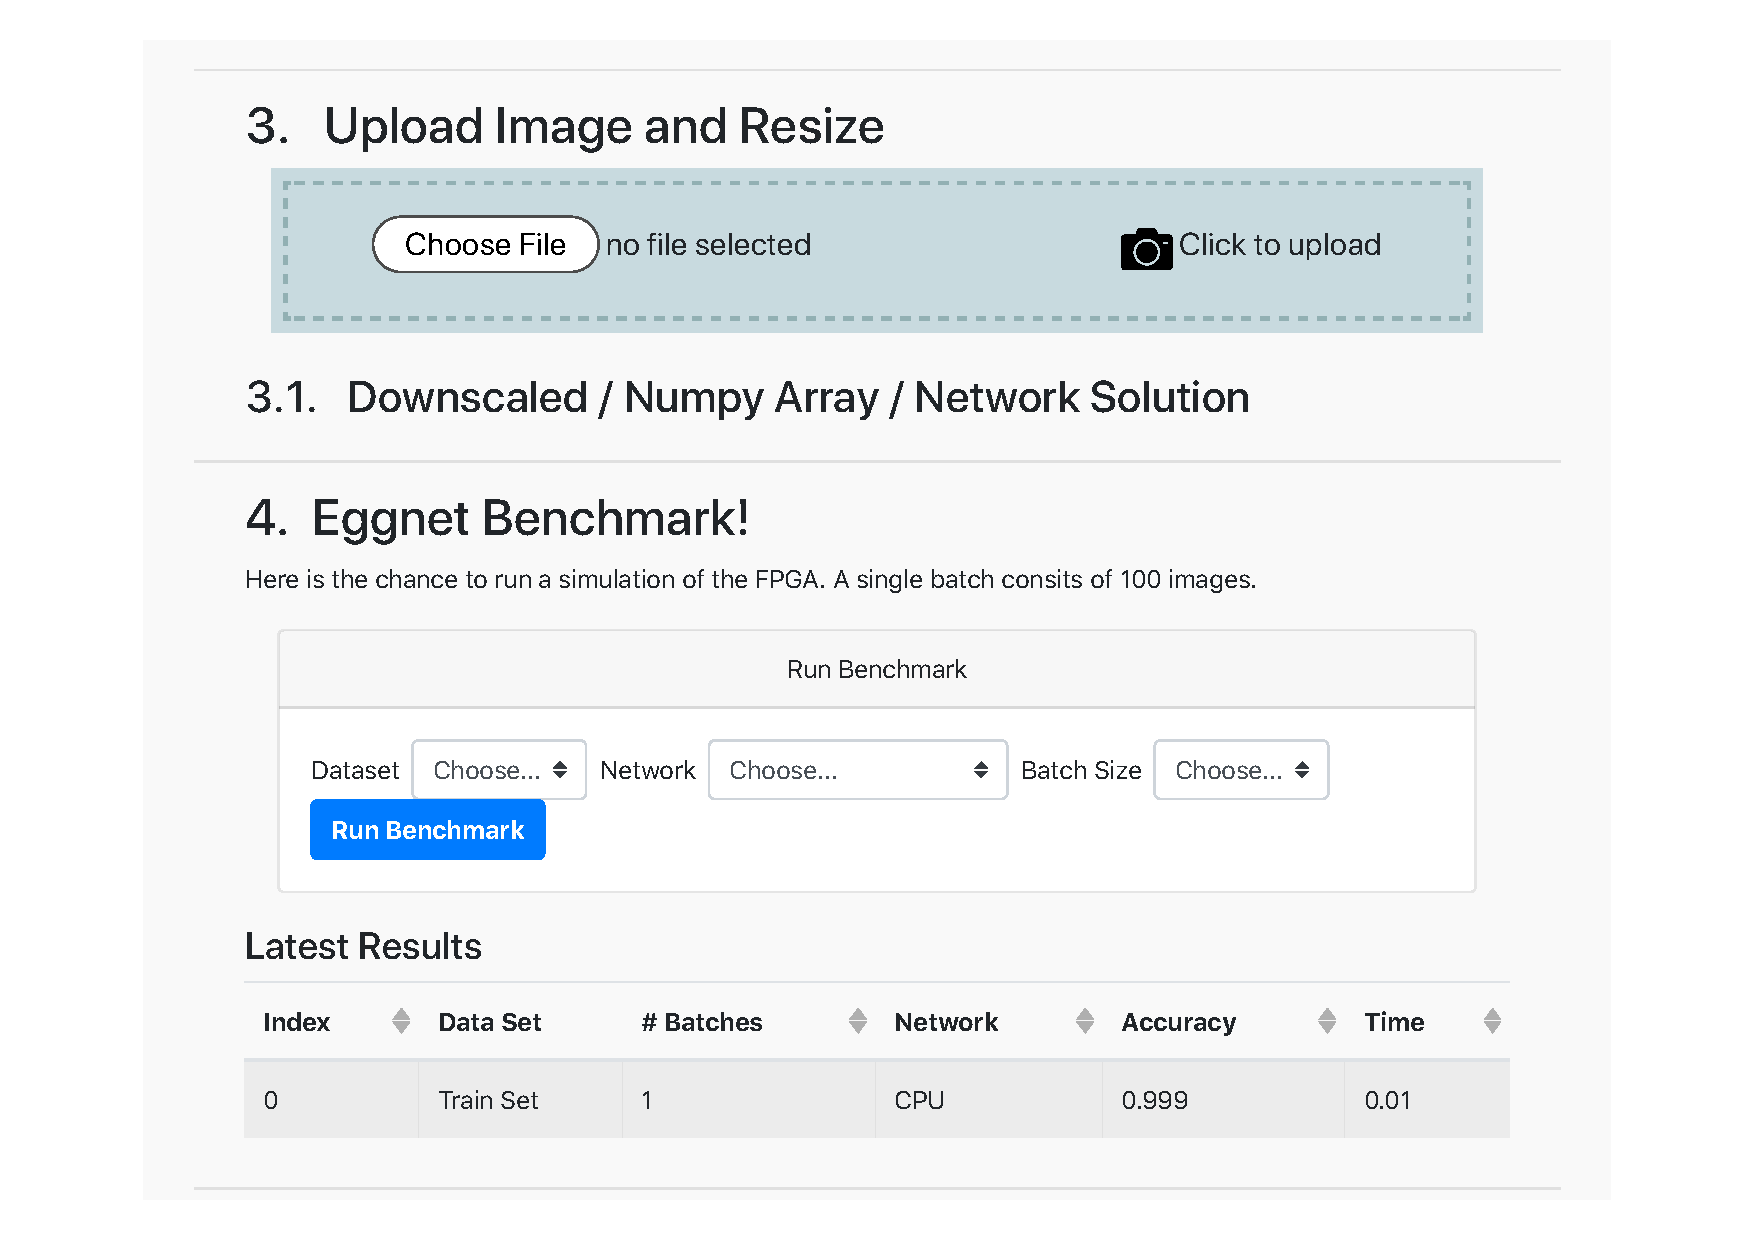
\includegraphics[width=0.8\textwidth]{img/webapp_bench}
  \caption{Screenshot of the Webapp's benchmark interface}
  \label{fig:sw-webapp-bench}
\end{figure}


\subsection{Build Software and Setup}

Additionally to the software needed for operating the network various tools are needed to actually \emph{build} the network itself. 
It is used for performing the training of the network and for generating a FPGA-bitstream based on the computed weights. Additionally the remote software is used to send the image data to the Zedboard and receive the results of the network for each image. 

Requirements of the Training Software:
\begin{itemize} 
	\item Training of the network considering bit resolution of implemented hardware
	\item Create VHDL code based on the network hyper-parameter and on the computed weights
	\item Create a bitstream with the generated VHDL code
\end{itemize}

Requirements of the Training Software:
\begin{itemize}
	\item Sends image data to Zedboard
	\item Receives results from Zedboard
	\item Create a figure of accuracy and performance   
	\item Optional: Send bitstream to hardware for partial reconfiguration
\end{itemize}

\subsubsection{Interface to Zedboard} \label{subsec:InterfaceRemoteZed}
As an interface to the Zedboard a flask application is running on the Zedboard which allows to upload a new image of a digit, test the hardware accelerate using the MNIST-dataset, gives useful information and allows to update the FPGA bitstream. 

